% Document setup
\RequirePackage{fix-cm}
\documentclass{article}
\usepackage{preamble}

%===============================%
%=============Inputs============%
%===============================%
\newcommand{\studentname}{Sharaf Hossain}

%===============================%
%====Make Solutions Visible=====%
%===============================%
\showsolutionstrue

%===============================%
%=============Figures===========%
%===============================%
% Remember to start figures with 

% \begin{figure}[H]

% the [H] is critical!


%==============================%
%=====Beginning of Document====%
%==============================%
\begin{document}
\pagestyle{mypagestyle}




%%%%%%%%%%%%%%%%%%%%%%%%%%%%%%%%%%%%%%%%%%%%%%%%%%%%%%%%%%%%%%%%%%%%%%%%%%%%%%%%%%%%%%%%%%%%%%%%%%%%%%%%%%%%%%%%%%%%%%%%%%
% PROJECT 8: NONLINEAR SYSTEM IDENTIFICATION FOR A CROP FIELD DIGITAL-TWIN
%%%%%%%%%%%%%%%%%%%%%%%%%%%%%%%%%%%%%%%%%%%%%%%%%%%%%%%%%%%%%%%%%%%%%%%%%%%%%%%%%%%%%%%%%%%%%%%%%%%%%%%%%%%%%%%%%%%%%%%%%%

\project{8}{Nonlinear System Identification for a Crop Field Digital-Twin}{Monday, May 4th  @ 11:59PM PST}

\textbf{Submission:}
\begin{enumerate}
    \item Submit the PDF copy of your typed report on Gradescope before the end of day (11:59 pm PST). 
    \item Submit your completed code to Gradescope. Failure to do so will result in 0 credit for the problems that require you to write code.
\end{enumerate}

\subsection*{Deliverables}
\begin{enumerate}

%%%%%%%%%%%%%%%%%%%%%%%%%%%%%%%
% Problem 1
%%%%%%%%%%%%%%%%%%%%%%%%%%%%%%%
\item[1. (a)] (10 points) Why is it important to evaluate our model, (say, in terms of mean squared error), on an unseen test set?

\begin{answer}
% %-----------------------------%
% % Place answer here
% %-----------------------------%
Evaluating on an unseen test set is essential because the genetic algorithm directly minimizes training error, making the training MSE an optimistically biased estimate of true model performance. A model can achieve low training MSE simply by overfitting to the noise and season-specific quirks of the training data rather than learning the underlying physical dynamics. If we reported only training error, we would have no way to distinguish a model that has genuinely recovered the growth parameters from one that has memorized irrelevant patterns. The held-out test season, which has independently generated forcing signals (different irrigation timing, fertilization schedule, and sunlight phase), provides an unbiased measure of how well the estimated parameters generalize to new conditions. A low test MSE gives us confidence that the recovered parameters reflect the true dynamics of the system, which is the actual goal of system identification.
\end{answer}
\newpage
\item[1. (b)] (25 points) Include an image of the generated train and test trajectories.

\begin{answer}
% %-----------------------------%
% % Place answer here
% \begin{figure}[H] will be helpful here
% %-----------------------------%
\begin{figure}[H]
    \centering
    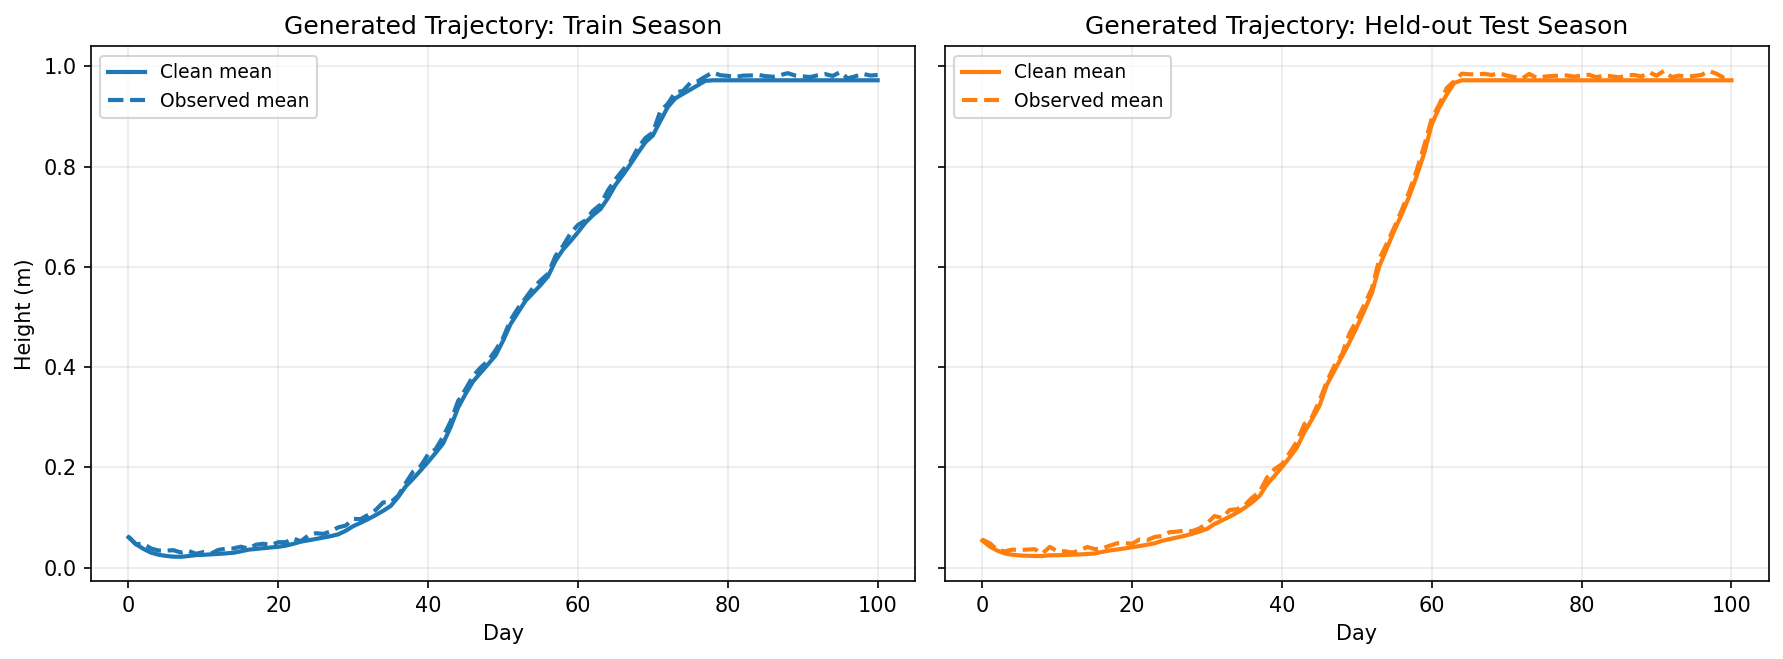
\includegraphics[width=\textwidth]{figures/trajectories.png}
    \caption{Mean plant height over a 100-day growing season. The clean (noiseless) trajectory and noisy observations are shown for the training season (left, blue) and the held-out test season (right, orange). Both seasons exhibit similar growth dynamics, with slight differences due to independently generated forcing signals (water, fertilizer, sunlight).}
    \label{fig:trajectories}
\end{figure}
\end{answer}
 \newpage 
%%%%%%%%%%%%%%%%%%%%%%%%%%%%%%%
% Problem 2
%%%%%%%%%%%%%%%%%%%%%%%%%%%%%%%
\item[2. (a)]  (15 points) Describe (just qualitatively, as we can't prove it numerically) how the increased number of parameters will impact our training error (i.e. lowest cost achieved with the GA). Will our model overfit or underfit the data?

\begin{answer}
% %-----------------------------%
% % Place answer here
% %-----------------------------%
In the current model, 7 parameters are shared across all 36 plants, reflecting the assumption that all plants obey the same underlying growth dynamics. If instead we fit a separate set of 7 parameters per plant, we have $7 \times 36 = 252$ free parameters. This dramatic increase in model capacity means the GA has far more degrees of freedom to shape each plant's predicted trajectory independently, and will therefore achieve a \textbf{lower training error}.

However, this comes at the cost of \textbf{overfitting}. With 252 parameters and only one season of training data, the model can assign each plant its own growth rate, competition strength, and input sensitivities in a way that perfectly explains the noisy observations of Season 1 — including the measurement noise — rather than the true shared dynamics. The fitted parameters would absorb season-specific noise rather than reflecting genuine physical relationships.

The consequence is that when this 252-parameter model is evaluated on the held-out test season, the test error will be substantially higher than the training error, because the plant-specific parameter values learned from Season 1 noise will not generalize to the different forcing conditions of Season 2. The shared 7-parameter model is preferable because it imposes the physically meaningful constraint that all plants follow the same growth law, which acts as a form of regularization and improves generalization.
\end{answer}
\newpage
\item[2. (b)] (10 points) How does the MSE error function differ from the cost function presented in Chapter 7 of the textbook?

\begin{answer}
% %-----------------------------%
% % Place answer here
% %-----------------------------%
The cost function from Chapter 7 of the textbook (Equations 7.7--7.8) is a \textbf{moment-matching} objective. Rather than comparing individual plant heights directly, it computes statistical moments of the entire canopy height distribution at each time frame --- the mean $M_1$, standard deviation $M_2$, skewness $M_3$, and kurtosis $M_4$ --- and measures how well the simulated moments match the observed ones:
\[
\Pi^{total}(\Lambda) = \frac{1}{N_f} \sum_{f=1}^{N_f} \left[ \sum_{i=1}^{N_d} w_i \, \Pi_i(\Lambda) \right]_f, \qquad \Pi_i(\Lambda) = \frac{\| M_i(\mathbf{h}) - M_i(\mathbf{h}^o) \|}{\| M_1(\mathbf{h}^o) \|}
\]
where $N_f$ is the number of time frames, $w_i$ are user-specified weights on each moment, and normalization is by $\|M_1(\mathbf{h}^o)\|$, the norm of the observed mean height.

The \texttt{normalized\_mse} used in this assignment differs in two fundamental ways. First, it is a \textbf{pointwise} comparison: it computes the mean squared error between each individual predicted and observed plant height at every timestep, rather than comparing aggregate distributional statistics. Second, it normalizes by the \textbf{variance} of the observed heights rather than by the first moment:
\[
\tilde{\Pi}(\Lambda) = \frac{\frac{1}{N}\sum_{k}\left( h_k^{\text{pred}} - h_k^{\text{obs}} \right)^2}{\text{Var}(\mathbf{h}^{\text{obs}}) + \varepsilon}
\]
In summary, the textbook objective matches the \emph{shape of the distribution} of canopy heights (via its moments), while this assignment's objective measures \emph{pointwise trajectory accuracy} across all plants and timesteps, normalized to be scale-invariant.
\end{answer}
\newpage
%%%%%%%%%%%%%%%%%%%%%%%%%%%%%%%
% Problem 3
%%%%%%%%%%%%%%%%%%%%%%%%%%%%%%%

\item[3. (a)]  (10 points) Include the plots of height trajectories for the train and test seasons. Include the parameter recovery table as well. Does the model generalize well when tested on the left-out set?

\begin{answer}
% %-----------------------------%
% % Place answer here
% %-----------------------------%
The GA was run with a population of 60, up to 200 generations, and early stopping after 30 generations without improvement. It converged in 187 generations.

\begin{figure}[H]
    \centering
    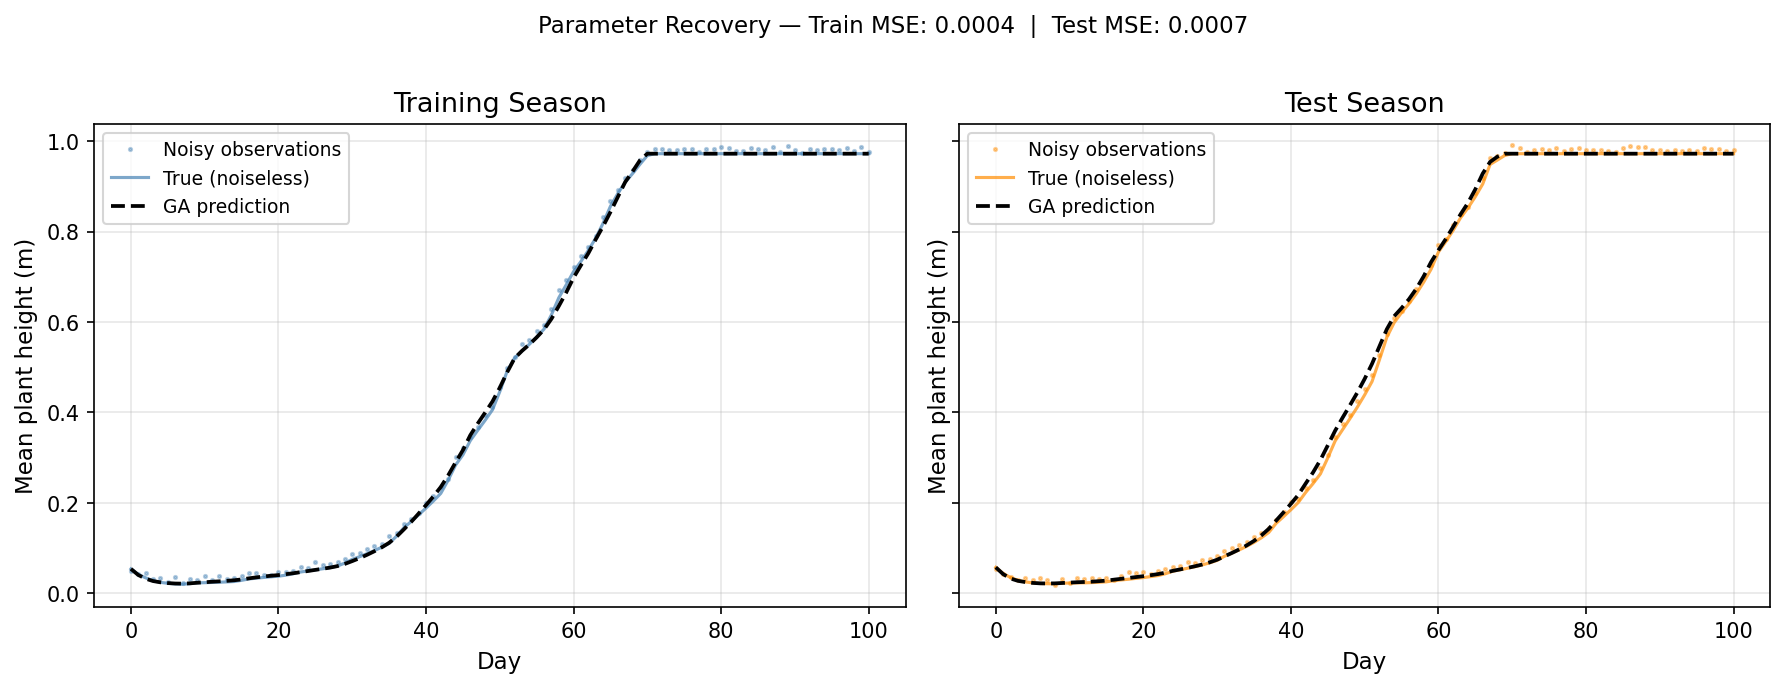
\includegraphics[width=\textwidth]{figures/trajectories_3a.png}
    \caption{Mean plant height over the 100-day growing season for the training season (left) and the held-out test season (right). The GA-recovered model (dashed black) closely tracks both the noiseless true trajectory and the noisy observations on both seasons.}
    \label{fig:trajectories_3a}
\end{figure}

\begin{table}[H]
\centering
\caption{Parameter recovery results. Train MSE = 0.0004, Test MSE = 0.0007.}
\begin{tabular}{lrrr}
\hline
\textbf{Parameter} & \textbf{True value} & \textbf{Recovered} & \textbf{\% Error} \\
\hline
$G_0$      & 0.1000 & 0.1223 & 22.3\% \\
$b_w$      & 0.5500 & 0.1000 & 81.8\% \\
$b_f$      & 0.3500 & 0.2036 & 41.8\% \\
$\gamma$   & 0.9000 & 1.2951 & 43.9\% \\
$\alpha$   & 0.9500 & 0.9511 &  0.1\% \\
$\lambda$  & 0.0800 & 0.0789 &  1.4\% \\
$\rho$     & 1.1000 & 1.0893 &  1.0\% \\
\hline
\end{tabular}
\label{tab:recovery}
\end{table}

Despite the poor pointwise recovery of $G_0$, $b_w$, $b_f$, and $\gamma$, the model generalizes well to the held-out test season: the test MSE (0.0007) is only slightly higher than the training MSE (0.0004), and both are very close to zero. The trajectory plot confirms that the GA-recovered model tracks the true growth dynamics accurately on an unseen season with independently generated forcing signals.
\end{answer}
\newpage
\item[3. (b)] (10 points) Which parameters are recovered accurately? Which are harder to identify, and why? Does this have a big impact on the predictive capability of our model?

\begin{answer}
% %-----------------------------%
% % Place answer here
% %-----------------------------%
Three parameters are recovered with high accuracy: $\alpha$ (0.1\% error), $\lambda$ (1.4\%), and $\rho$ (1.0\%). Four parameters are recovered poorly: $b_w$ (81.8\%), $b_f$ (41.8\%), $\gamma$ (43.9\%), and $G_0$ (22.3\%).

The reason for the poor recovery of $G_0$, $b_w$, $b_f$, and $\gamma$ is \textbf{structural non-identifiability}. All four parameters appear exclusively inside the combined effective growth factor
\[
G(t) = G_0 \bigl(1 + b_w W(t) + b_f F(t)\bigr) \, S(t)^{\gamma}.
\]
The trajectory $h(t)$ depends on this product as a whole, not on each factor individually. As a result, there exist infinitely many combinations of $\{G_0, b_w, b_f, \gamma\}$ that yield the same effective $G(t)$ and therefore the same predicted heights. The GA correctly finds a parameter set that minimizes the MSE, but it cannot distinguish between the many equally valid combinations of these four parameters. This is a fundamental property of the model structure, not a limitation of the GA.

By contrast, $\alpha$ appears as the exponent on plant height ($h^\alpha$), $\lambda$ scales the competition term independently of the growth term, and $\rho$ controls the spatial decay of inter-plant interactions. These parameters have structurally distinct effects on the dynamics that cannot be compensated by adjusting the others, making them uniquely identifiable from the trajectory data.

Despite the large errors in $\{G_0, b_w, b_f, \gamma\}$, the impact on predictive capability is limited under similar forcing conditions. Since the recovered parameters produce an effective $G(t)$ that closely matches the true one, the model still predicts plant growth accurately, as confirmed by the near-zero test MSE (0.0007). However, if the forcing signals were to change dramatically beyond the range seen in training --- for example, a season with much higher water or fertilizer inputs --- the model could fail, because the individually incorrect $b_w$ and $b_f$ would produce the wrong sensitivity to those inputs even if their combined effect happened to match in the training regime.
\end{answer}
\newpage
\item[3. (c)] (20 points) Generate new data by increasing the \texttt{noise\_sigma} parameter of \texttt{generate\_dataset} and report your parameter recovery table after running the GA on this new data. How does increasing the noise level of our model impact our ability to recover parameters accurately?

\begin{answer}
% %-----------------------------%
% % Place answer here
% %-----------------------------%
The dataset was regenerated with \texttt{noise\_sigma = 0.20} (increased from 0.03). The GA was run with identical hyperparameters and converged in 144 generations.

\begin{figure}[H]
    \centering
    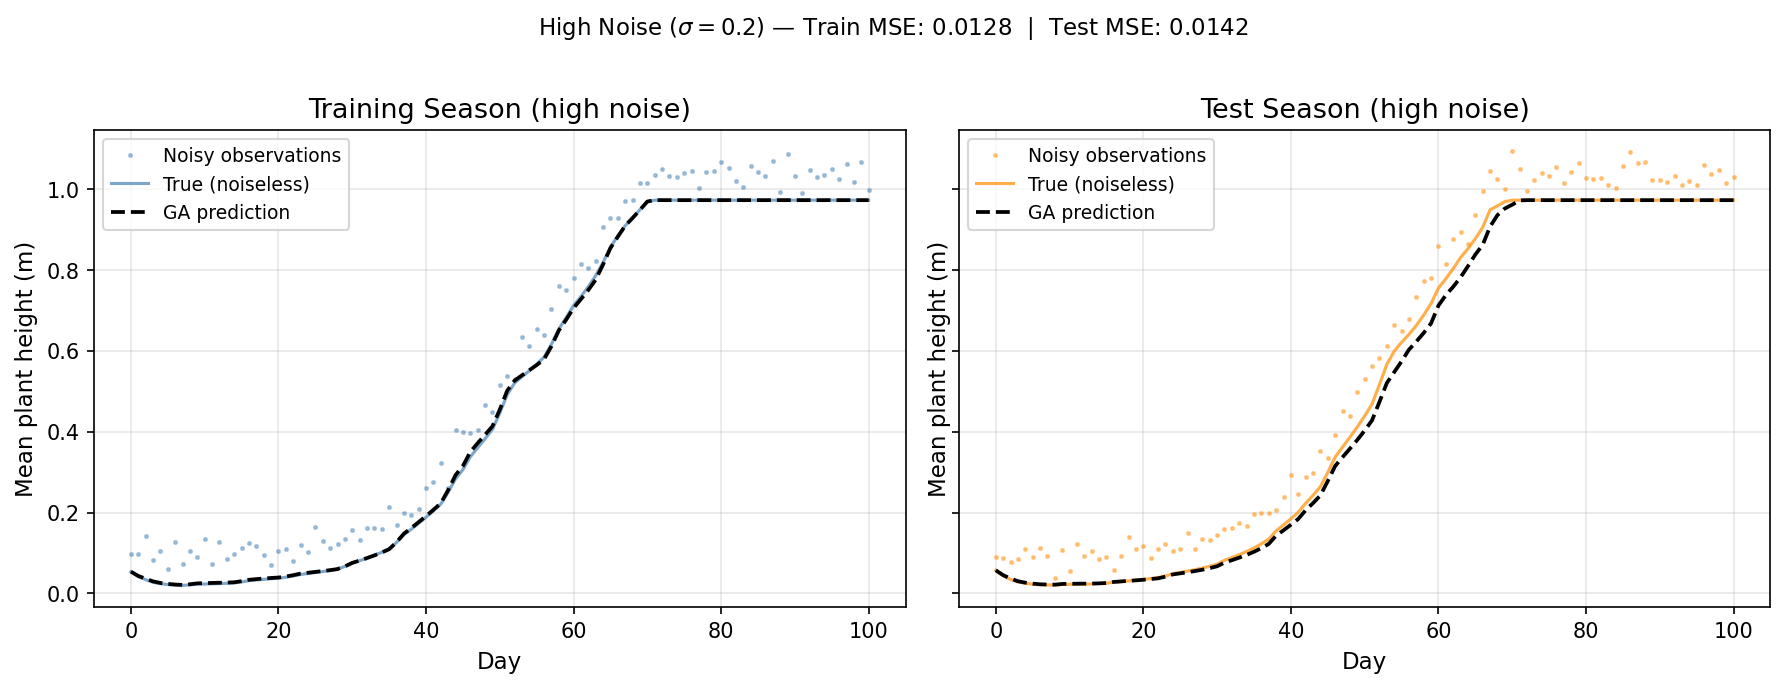
\includegraphics[width=\textwidth]{figures/trajectories_3c.png}
    \caption{Mean plant height trajectories under high noise ($\sigma = 0.20$). The noisy observations scatter much more widely around the true trajectory, making it harder for the GA to isolate the underlying dynamics.}
    \label{fig:trajectories_3c}
\end{figure}

\begin{table}[H]
\centering
\caption{Parameter recovery comparison: low noise ($\sigma=0.03$) vs.\ high noise ($\sigma=0.20$).}
\begin{tabular}{lrrrr}
\hline
\textbf{Parameter} & \textbf{True} & \textbf{Recovered ($\sigma$=0.03)} & \textbf{Recovered ($\sigma$=0.20)} & \textbf{\% Error ($\sigma$=0.20)} \\
\hline
$G_0$      & 0.1000 & 0.1223 & 0.0988 &  1.2\% \\
$b_w$      & 0.5500 & 0.1000 & 0.7375 & 34.1\% \\
$b_f$      & 0.3500 & 0.2036 & 0.5056 & 44.5\% \\
$\gamma$   & 0.9000 & 1.2951 & 1.0838 & 20.4\% \\
$\alpha$   & 0.9500 & 0.9511 & 0.9536 &  0.4\% \\
$\lambda$  & 0.0800 & 0.0789 & 0.0761 &  4.9\% \\
$\rho$     & 1.1000 & 1.0893 & 1.0788 &  1.9\% \\
\hline
Train MSE & --- & 0.0004 & 0.0128 & --- \\
Test MSE  & --- & 0.0007 & 0.0142 & --- \\
\hline
\end{tabular}
\label{tab:recovery_noise}
\end{table}

Increasing the noise level has two main effects. First, the MSE values rise substantially (train MSE: $0.0004 \to 0.0128$; test MSE: $0.0007 \to 0.0142$), since the noisy observations provide a less informative training signal and the GA is fitting a noisier target. Second, individual parameter recovery becomes less consistent. The structurally identifiable parameters $\alpha$, $\lambda$, and $\rho$ remain well recovered under high noise (errors below 5\%), because their roles in the ODE are geometrically distinct. However, the non-identifiable group $\{G_0, b_w, b_f, \gamma\}$ shifts to a different equally valid combination under high noise: for example, $b_w$ moves from 0.10 to 0.74 across the two runs, reflecting the fact that the GA converges to a different point in the flat region of the loss landscape.

Crucially, the generalization gap remains small under high noise (test MSE $-$ train MSE $= 0.0014$), indicating that the model still captures the dominant growth dynamics rather than overfitting to noise. However, the absolute MSE values are much higher than in the low-noise case, meaning predictions are less accurate. This demonstrates that noise degrades the quality of the recovered model even when it does not cause overfitting.
\end{answer}

\end{enumerate}
% End document
\end{document}